\section{Introduction}

\begin{frame}
\tableofcontents[currentsection, hideothersubsections]
\end{frame}

\begin{frame}{Problématique}
	\begin{alertblock}{AVC : Constat}
		Un individu sur 600 est victime d'un AVC chaque année. \\
		120 000 AVC/an en France. \\ \pause 
		Cause fréquente d'hémiplégie chez les victimes. \\
		Une des principales causes d'invalidité.
	\end{alertblock}
\end{frame}

\begin{frame}{La réponse actuelle}
	\begin{block}{Pour le patient}
	Des programmes et séances de réhabilitations.\\
	Des tests de mesure des capacités sensorimotrices :
		\begin{itemize}
			\item Tests de déficiences
			\item Tests fonctionnels
		\end{itemize}
	\end{block}
\end{frame}

\begin{frame}
	\begin{block}{Les outils standards}
		Un test de déficiences: le score de Fugl Meyer \\
		Un instrument de mesure des angles : le goniomètre
		\end{block}
		\begin{center}
			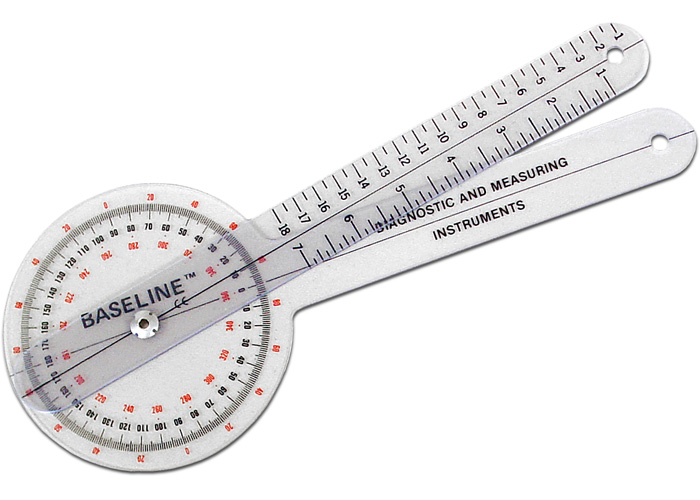
\includegraphics[width=4cm]{../images/goniometre.jpg}
			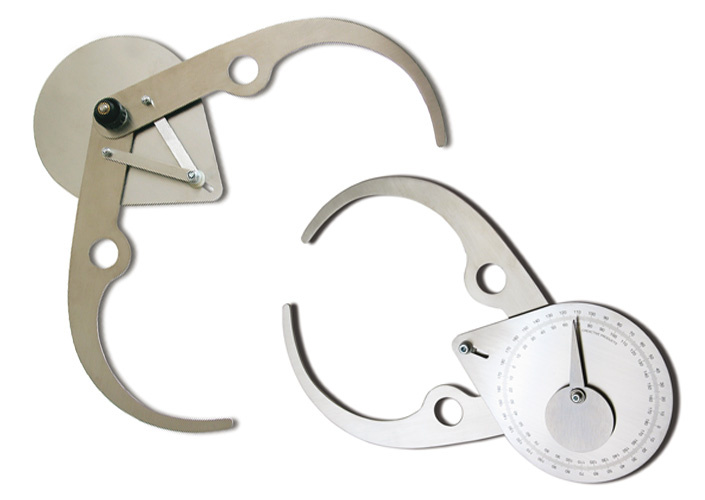
\includegraphics[width=4cm]{../images/clockprop.jpg}
	\end{center}
\end{frame}

\begin{frame}{La réponse actuelle}
\begin{block}{Limites}
Le test de FM nécessite des mesures d'angles précises.\\
Le temps de réalisation du test : 45min \\ \pause
Le goniomètre se révèle :
\begin{itemize}
	\item intrusif
	\item imprécis
	\item finalement souvent délaissé
\end{itemize}
\end{block}
\end{frame}

\begin{frame}{Problématique}
\begin{block}{Piste de réflexion}
Dans quelle mesure l'outil informatique peut il apporter quelque chose dans la réalisation d'un test de FM?
\end{block}
\end{frame}
